
%(BEGIN_QUESTION)
% Copyright 2006, Tony R. Kuphaldt, released under the Creative Commons Attribution License (v 1.0)
% This means you may do almost anything with this work of mine, so long as you give me proper credit

Hva er en ventil-{\it aktuator}? Hva betyr det hvis en glidespindel-ventilaktuator er {\it reversvirkende}? Hvordan skiller dette seg fra en {\it direktevirkende} aktuator?

\underbar{file i00779}
%(END_QUESTION)





%(BEGIN_ANSWER)

En ventil-{\it aktuator} er mekanismen som beveger ventilspindel eller aksel som respons på et styresignal, vanligvis trykkluft.

\vskip 10pt

En {\it reversvirkende} ventilaktuator er en aktuator der aktuatorstangen trekkes inn i aktuatoren (trekkes opp fra ventilhuset) når lufttrykk påføres:

$$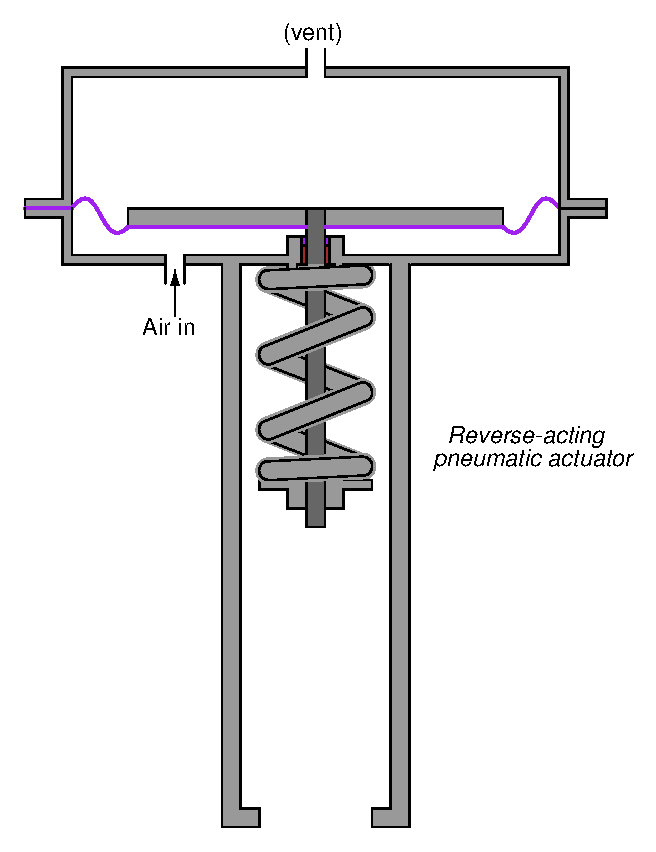
\includegraphics[width=15.5cm]{i00779x01.eps}$$

I motsetning til dette vil en {\it direktevirkende} aktuator skyve stangen ut (inn i ventilhuset) når lufttrykk påføres:

$$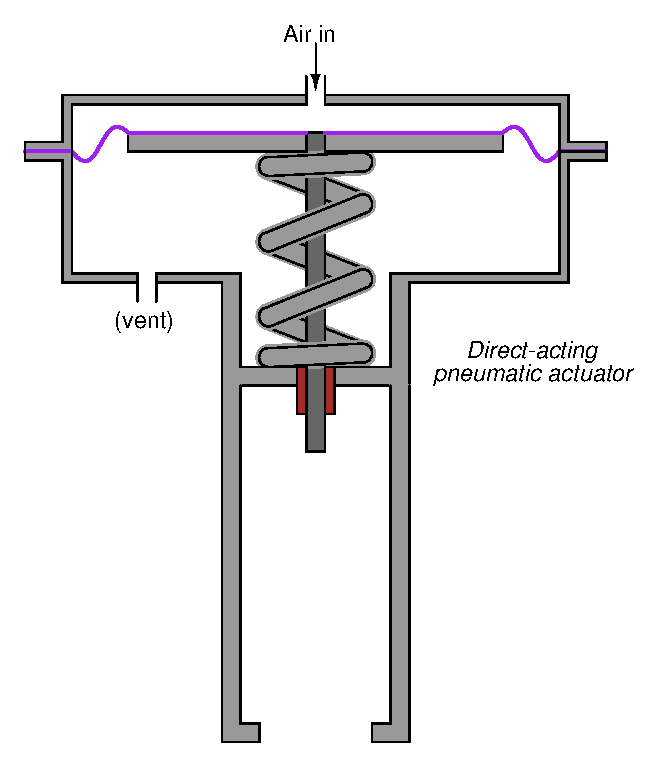
\includegraphics[width=15.5cm]{i00779x02.eps}$$

%(END_ANSWER)





%(BEGIN_NOTES)

Aktuatorer finnes i flere varianter, vanligvis pneumatiske. Men hydrauliske og elektriske aktuatorer finnes også, med ulike fordeler og ulemper sammenlignet med mer vanlige pneumatiske løsninger.

En huskeregel jeg bruker for direkte/revers-forholdet er enkelhet i design. En direktevirkende aktuator trenger ingen tetning rundt stangen, og er derfor enklere enn en reversvirkende aktuator. Når du ser ordet «direkte», tenk {\it enkel}.

%INDEX% Sluttkontrollelementer, ventil: direktevirkende og reversvirkende aktuator

%(END_NOTES)


